\documentclass [11pt]{article}
\usepackage{amsmath,amssymb,amsfonts,epsfig,algorithm,algorithmic,url, mathtools, indentfirst, color, soul}

\textheight 8.8truein
\parskip 0.1in
\topmargin -0.5truein
\textwidth 6.5truein
\oddsidemargin -0.05in
\evensidemargin -0.05in
% \renewcommand{\baselinestretch}{1.2}   %line space adjusted here
\setcounter{footnote}{0}
\sloppy

\renewcommand{\theequation}{\thesection.\arabic{equation}}
\newcommand{\newsection}{\setcounter{equation}{0}\section}

% redefining commonly used symbols
\DeclareMathOperator{\trace}{Tr}

\newtheorem{theorem}{Theorem}
\newtheorem{proposition}[theorem]{Proposition}
\newtheorem{lemma}[theorem]{Lemma}
\newtheorem{corollary}[theorem]{Corollary}
\newtheorem{definition}[theorem]{Definition}
\newtheorem{example}[theorem]{Example}


\title{\textbf{EE394V Data Analytics in Power Systems\\\medskip Learning for DC-OPF: Classifying Active Constraints using Graph Attention Nets}}
\author{JeeHyun Park\\University of Texas at Austin}

\begin{document}

\maketitle
\nocite{*}


\begin{abstract}
Optimal power flow (OPF) is used in power system operational planning to estimate the most economical efficiency solution while satisfying demand and safety margins. 
Due to increasing uncertainty and variability in energy sources and demand, the optimal solution needs to be updated near real-time to respond to observed uncertainty realizations. 
There was an approach to solving optimal power flow problems. However, it took significant time to train the model and allows us any interpretability between input and output features. 
In this paper, we propose the use of Graph Attention Network as an OPF problem-solver, which has a short training time and interpretability.

\end{abstract}


%%%%%%%%%%%%%%%%%%%%%%%%%%%%%%%%%%%%
% Introduction
%%%%%%%%%%%%%%%%%%%%%%%%%%%%%%%%%%%%
\section{Introduction}

Optimal power flow (OPF) is used in power system operational planning to estimate the most economical efficiency solution while satisfying demand and safety margins.

Due to increasing uncertainty and variability in energy sources and demand, the optimal solution needs to be updated near real-time to respond to observed uncertainty realizations ($\omega$).

The existing methods, such as affine control policy and ensemble control policy, could not cope with frequent updating due to the high computational complexity. As a result, an approach to solving optimal power flow problems using neural networks \cite{DC_OPF_NNs} was presented. 
The method has succeeded in significantly lowering computational complexity, but it took a significant amount of time to train the model due to a large number of training parameters. Moreover, due to the characteristic of neural nets, there is no room to interpret any relationship between input and output features. 

Through this project, we propose to use the model based on Graph Attention Networks (GAT)\cite{GAT}, which requires less training parameters and has interpretability between input and output features.

%%%%%%%%%%%%%%%%%%%%%%%%%%%%%%%%%%%%
% Problem Formulation
%%%%%%%%%%%%%%%%%%%%%%%%%%%%%%%%%%%%
\section{Problem Formulation}

\subsection{OPF and Graph Attention Networks Model}

\subsubsection{Object of the model}

We will build models that takes uncertainty realizations ($\omega$) as input and outputs the active constraints.

\begin{itemize}
  \item Input: a vector ($\omega$) corresponding to uncertainty realizations of active demand power at every nodes.
  \item Output: a vector indicating whether the constraints are active or not (1 or 0).
\end{itemize}

\subsubsection{Why Graph based model?}

The graph neural network (GNN) \cite{GNN} based model configures training parameters based on the topology of a given power system. As a result, it can be trained through \textbf{fewer training parameters} than the neural network based model.

\subsubsection{Why do we need Attention?}

The purpose of attention is to improve the performance of the model by determining which input features are critical. In addition to improving performance, we can \textbf{track the relationship between input and output} by analyzing attention weights.


%%%%%%%%%%%%%%%%%%%%%%%%%%%%%%%%%%%%
% Numerical Experiments
%%%%%%%%%%%%%%%%%%%%%%%%%%%%%%%%%%%%
\section{Numerical Experiments}

% \begin{itemize}
%   \item Input: 
%   \item Output: 
% \end{itemize}


\subsection{Dataset}

We will use the data provided by the IEEE PES PGLib-OPF Benchmark Library\cite{power-grid-lib}. Moreover, we will generate feasible sets of uncertainty realizations and active constraints through Matpower\cite{matpower}. 


\subsection{Models}

\begin{itemize}
  \item Neural Nets based model (Baseline)
  \item Graph Neural Nets(GNN) based model
  \item Graph Attention Nets(GAT) based model
\end{itemize}

We hope to see the GNN based model shows better performance than the baseline, and the GAT based model shows the best. Moreover, we hope to visualize the attention weight parameters as the Figure~\ref{fig:eg vis}, which will allow us to have better interpretability.

\begin{figure}[h]

\end{figure}


\begin{figure}[ht]
	\centering
	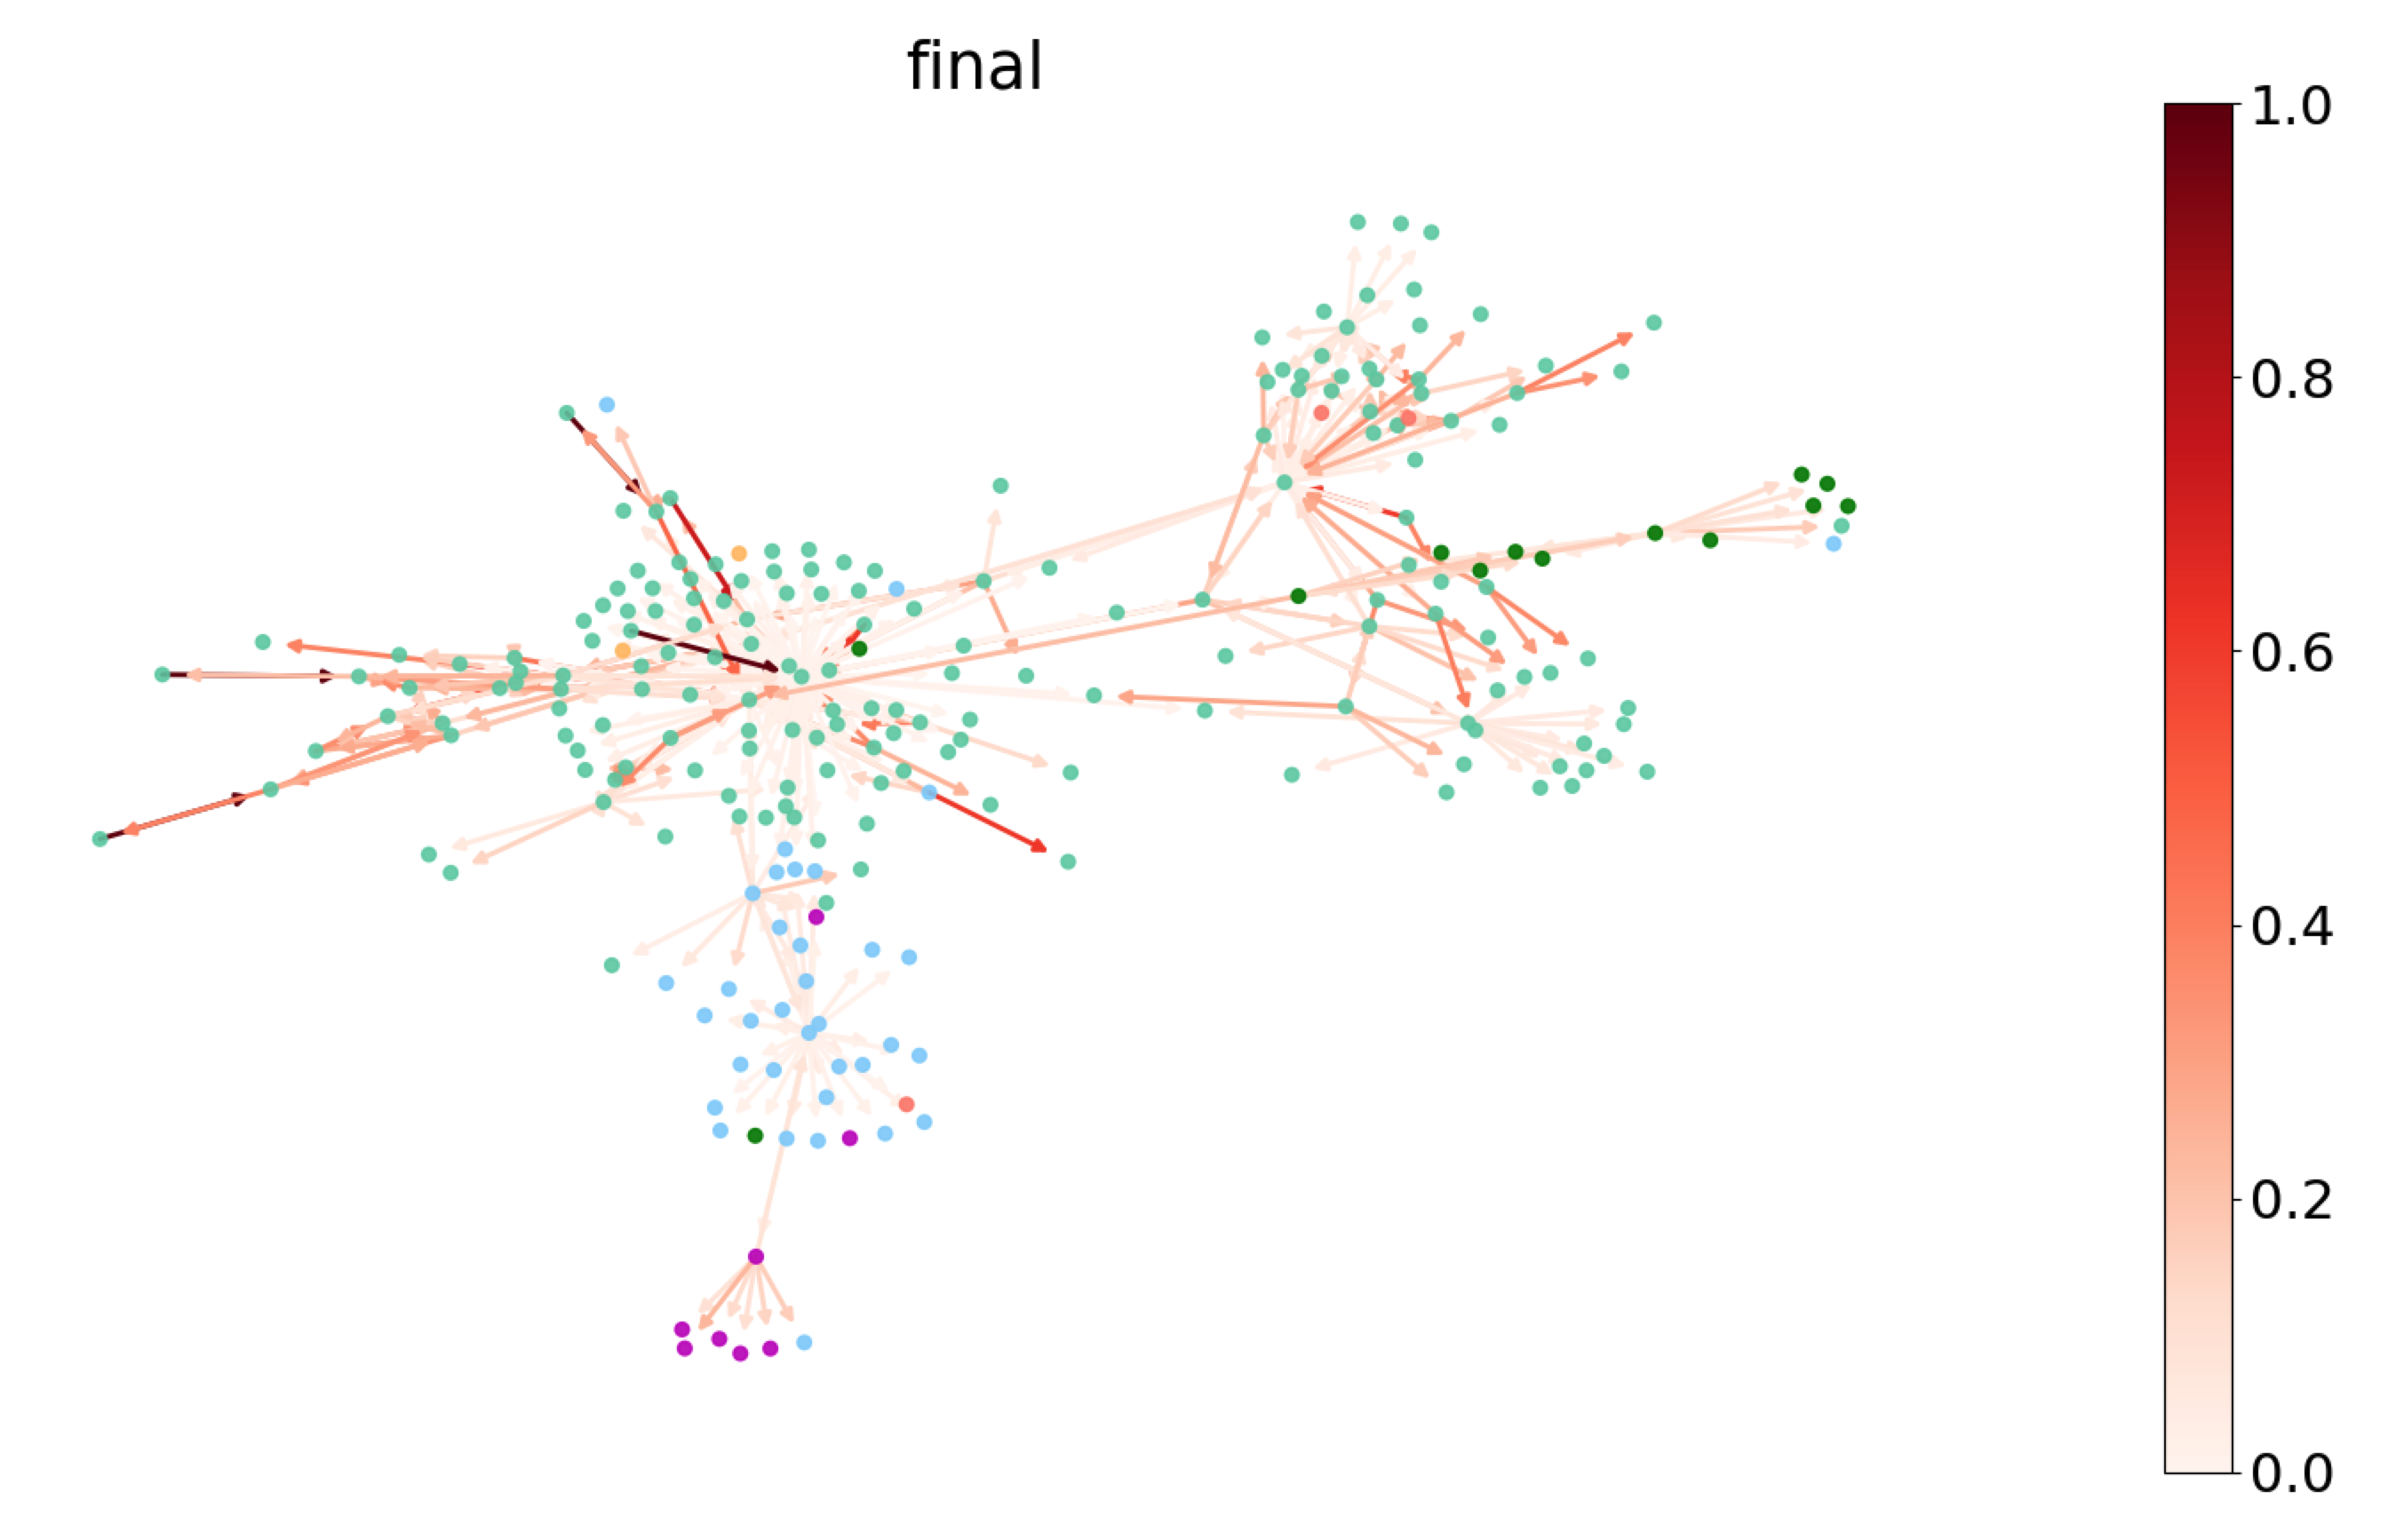
\includegraphics[scale=0.1]{etc/proposal/figures/eg of visualize gat attention weights.png}
	\caption{Example of visualization of GAT attention weights\cite{gat_eg}}
    \label{fig:eg vis}
\end{figure}

%%%%%%%%%%%%%%%%%%%%%%%%%%%%%%%%%%%%
% Concluding Remarks
%%%%%%%%%%%%%%%%%%%%%%%%%%%%%%%%%%%%
\section{Concluding Remarks}

We hope to have the result that GAT based model shows the best performance and better interpretability by analyzing the attention weights.

\bibliographystyle{IEEEannot}
\bibliography{annot}
\end{document}